\documentclass{article}
% Language setting
% Replace `english' with e.g. `spanish' to change the document language
\usepackage[english]{babel}

% Set page size and margins
% Replace `letterpaper' with `a4paper' for UK/EU standard size
\usepackage[letterpaper,top=2cm,bottom=2cm,left=3cm,right=3cm,marginparwidth=1.75cm]{geometry}

% Useful packages
\usepackage{amsmath}
\usepackage{graphicx}
\usepackage[colorlinks=true, allcolors=blue]{hyperref}
\usepackage{adjustbox}
\usepackage{pgffor}
\usepackage{graphicx}
\usepackage{xcolor}
\newadjustimage{\myimage}{max size={.33\textwidth}{.33\textwidth}}%
\usepackage{caption}
\usepackage{listings}
\usepackage{subcaption}
\usepackage{braket}
\usepackage{dsfont}
\usepackage{float}
\usepackage{indentfirst}

\usepackage[
backend=biber,
sorting=ynt
]{biblatex}
\addbibresource{references.bib}


%--------------------------------   NAO MEXER ACIMA

\begin{document}

%\maketitle     %(antigo)

\begin{titlepage}
	\centering
	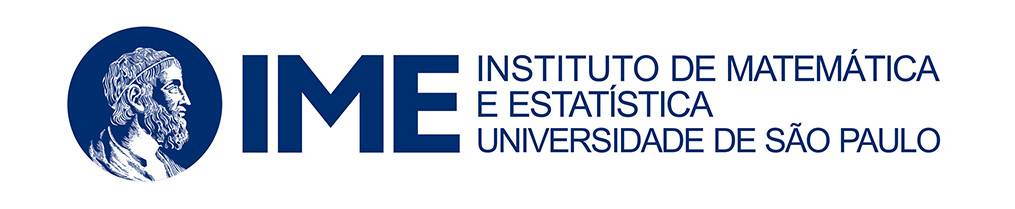
\includegraphics[width=0.8\textwidth]{images/logo_ime.png}\par
	\vspace{2cm}
 
	% {\scshape\LARGE Relatório Científico do projeto na modalidade Bolsa de Iniciação Científica, fomentado pela Fundação de Amparo à Pesquisa do Estado de São Paulo. \par}

	%%%% PROJECT TITLE
	{\huge\bfseries Quantum Walks and its Applications in Quantum Networks  \par}
	\vspace{2cm}

     
\includegraphics[width=0.5\textwidth]{images/umass_logo.png}\par
	\vspace{3cm}
	
	%%%% AUTHOR(S)
	{\Large Undergraduate Thesis - Andre Nogueira Ribeiro}\par
    {\Large Supervisor: Prof. Fabio Kon (IME/USP)}\par
    {\Large Co-supervisor:  Prof. Antonio Jorge Gomes Abelém (UFPA)}\par
    {\Large Supervisor at University of Massachusetts: Prof. Don Towsley(UMass)}\par
	\vspace{1.5cm}
 
\end{titlepage}

\newpage

\tableofcontents

\section{Abstract}
    Quantum computing emerged from the idea of building a machine capable of simulating complex quantum systems, a concept proposed by physicist Richard Feynman and mathematician Yuri Manin. The challenge with simulating quantum systems on classical computers is that the computational effort increases exponentially with the size of the system, making it impractical for any significantly large problems. In addition to this focus, research in quantum algorithms has also achieved notable success, with algorithms with better complexity than classical ones being proposed—such as Shor's algorithm for number factorization.

    Quantum computing is also an exciting field of study, offering a wide range of unexplored possibilities, which makes it both intriguing and promising. Currently, companies like Google and IBM, have developed functional quantum machines that highlight the importance of this technology. These machines are capable of performing computations that are inaccessible to classical computers due to their distinct physical properties. Some of the main challenges in advancing quantum computers include increasing the number of qubits (the basic unit of memory in quantum computing), reducing noise, and extending coherence time (the duration of quantum phenomena needed to execute an algorithm).

\section{Introduction to Quantum Computing}

\paragraph{Qubit} A qubit is the fundamental unit of memory in a quantum computer, and unlike classical bits, it can exist in more than just the 0 or 1 states. Thanks to quantum properties, a qubit can exist in a superposition of both 0 and 1, in infinitely many different forms. However, these infinite states exist only before measurement. When the state of a qubit is measured, the result is either 0 or 1, meaning the qubit "collapses" (the more technical term) to one of these two states. It is possible to harness the computational power of these infinite states without directly measuring them, which leads to a significant computational advantage.

\paragraph{Mathematical Model.} By studying the literature, particularly chapter 2.1 of the book Quantum Computation and Quantum Information, which reviews the necessary linear algebra to understand the mathematical model used in quantum computing, I explored the theory behind the representation of a quantum computing system. A qubit, the basic memory unit of a quantum computer, can be represented as a two-dimensional vector, and the quantum gates that act on this qubit can be represented by unitary matrices.

The state of a qubit can be written as $v = a\ket{0} + b\ket{1}$, where $\ket{0}$ is the vector (1,0), representing the state with a probability of 1 to collapse to 0, and $\ket{1}$ is the vector (0,1), representing the state with a probability of 1 to collapse to 1. The value $|a|^2$ is the probability that the qubit will be 0 after measurement, and $|b|^2$ is the probability that it will be 1. Naturally, for this to work, $|a|^2 + |b|^2$ must equal 1.

It is worth noting that often multiple qubits are considered together, and this is represented by a vector with more dimensions. Each additional qubit doubles the number of dimensions. For example, a system of 2 qubits is represented by a 4-dimensional vector.

There is also a common representation called the Bloch sphere, which visualizes the qubit as a 3D vector, also including the global phase of the qubit (a physical property associated with it). In this section, it was also necessary to understand the probabilistic relationships involved in this context.

\paragraph{Quantum Gates} 

In a circuit, a gate is responsible for changing the information that passes through it in a specific way. In quantum computing, gates are represented by square unitary matrices (a gate acting on one qubit is a 2x2 unitary matrix, while a gate acting on two qubits is a 4x4 unitary matrix).

Some of the quantum gates studied include the Hadamard gate, which creates a superposition of states with equal probability; the X gate, which flips the probabilities of measuring 0 and 1 in a qubit; and the CNOT gate, which acts on two qubits such that, depending on the state of one (called the control qubit), it affects or does not affect the other (called the target qubit). Other gates studied include the Toffoli gate, the Phase gate, and the T gate.

The matrix representations of some of these gates were presented. Understanding these gates was essential for later understanding more complex quantum circuits.
    
\section{Quantum Algorithms}

\section{Introduction to Quantum Information}

\section{Introduction to Quantum Walks}

\section{Distributed Quantum Walk Control Plane for Quantum Networks}

\section{Future Possibilities}

\pagebreak
\printbibliography[]
\end{document}